\documentclass[9pt,twocolumn,twoside,lineno]{pnas-new}
% Use the lineno option to display guide line numbers if required.

%not sure where to put this - Ofelia
\usepackage{svg}
\usepackage{subfig}

\templatetype{pnasresearcharticle} % Choose template 
% {pnasresearcharticle} = Template for a two-column research article
% {pnasmathematics} %= Template for a one-column mathematics article
% {pnasinvited} %= Template for a PNAS invited submission


%\include{subfigure}
%\usepackage{amssymb, amsmath, amsfonts}
%\usepackage{bm}
%\usepackage{multirow}
%\usepackage{graphicx}
%\usepackage{comment}
%To be removed
%\usepackage[normalem]{ulem} %To be removed
%\usepackage[usenames,dvipsnames]{color}
%To be removed
%\usepackage{subfig}
%\graphicspath{ {images/}{./Tex//} }


%\newcommand{\DFcomment}[1]{\textbf{\color{blue}([DF:]}
%\textbf{\color{blue} #1} \textbf{\color{blue}) }}
%\providecommand{\red}[1]{\textcolor{red}{#1}}
%\definecolor{darkgreen}{rgb}{0.1, 0.5, 0.1}
%\providecommand{\green}[1]{\textcolor{darkgreen}{#1}}

\definecolor{mygreen1}{RGB}{68,120,33}
\definecolor{mygreen21}{RGB}{141,211,95}
\definecolor{mygreen22}{rgb}{0.413,0.596,0.293}
\definecolor{mygreen23}{rgb}{0.273,0.365,0.213}
\definecolor{mygreen24}{rgb}{0.133,0.133,0.133}
\definecolor{mypink1}{RGB}{255,179,128}
\definecolor{mypink2}{rgb}{0.782,0.559,0.409}
\definecolor{mypink3}{rgb}{0.565,0.417,0.317}
%\definecolor{myyellow}{RGB}{255,221,85}
%\definecolor{mygrey}{RGB}{179,179,179}
\newcommand{\legendline}[1]{{\color{#1} \rule[1pt]{8pt}{2.5pt}}}
\newcommand{\legenddot}[1]{{\color{#1} $\bullet$}}
\newcommand{\legenddash}[1]{{\color{#1} \rule[1pt]{3.5pt}{1.5pt}\,\rule[1pt]{3.5pt}{1.5pt}}}
\newcolumntype{M}{>{\raggedright\arraybackslash}p{3.6cm}}
\newcolumntype{T}{>{\raggedright\arraybackslash}p{8.6cm}}
%\renewcommand{\arraystretch}{1.8}




%\title{A population dynamics model for catheter-associated urinary tract infections}
%\title{Urine production rate is critical in a model for catheter-associated urinary tract infection}
%\title{Spatial partitioning enhances collective antibiotic resistance}
\title{Spatial partitioning of a microbial population enhances collective enzymatic benefits} 
%???defence ? but also resource foraging?

\author[a,b,c]{Nia Verdon}
\author[c]{Ofelia Popescu}
\author[c]{Simon Titmuss}
\author[a,b,c]{Rosalind J. Allen}


\affil[a]{Theoretical Microbial Ecology, Institute of Microbiology, Faculty of Biological Sciences, Friedrich Schiller University Jena, Jena, Germany}
\affil[b]{Cluster of Excellence Balance of the Microverse, Friedrich Schiller University Jena, Jena, Germany}
\affil[c]{School of Physics and Astronomy, University of Edinburgh, Edinburgh, UK}
\affil[d]{School of Physics and Astronomy, University of Edinburgh, Edinburgh, UK}





%\leadauthor{Bull} 

\significancestatement{xxx
}  

\authorcontributions{
All authors designed the study; NV and OP performed the calculations, computations and analysed the data; all authors discussed the results; all authors wrote and edited the manuscript. }
\authordeclaration{Authors declare no conflicts of interest}

\correspondingauthor{\textsuperscript{1}To whom correspondence should be addressed. E-mail: rosalind.allen@uni-jena.de; simon.titmuss@ed.ac.uk}

\keywords{population dynamics $|$  spatial partitioning $|$ collective defence $|$ social trait $|$ beta-lactamase  $|$ inoculum effect  $|$ stochasticity} 

\begin{abstract}
In the natural environment, microbes often produce enzymes that modify their local environment. This can produce collective benefits such as removal of antibiotic or release of environmental nutrients. Spatial partitioning is a common feature of many microbial environments and plays a central role in the theory of social trait evolution.  Here, we show theoretically that, even for a clonal population of enzyme producers, spatial partitioning into multiple small populations can strongly enhance the collective benefits of enzymatic environment modification. For the clinically relevant case where beta-lactamase producing bacteria mount a collective defence against antibiotic via enzymatic degradation, we show that partitioned populations can survive antibiotic concentrations that would be sufficient to kill a non-partitioned population. For a model of collective enzymatic nutrient foraging, spatial partitioning can enhance total population growth compared to an unpartitioned population. This "partitioning enhancement" is a purely stochastic effect, originating from variation in the initial bacterial densities among different subpopulations.  Our results have  implications for the development of effective antibiotic treatment protocols for strongly partitioned infections. 
\end{abstract}

\dates{This manuscript was compiled on \today}
\doi{\url{www.pnas.org/cgi/doi/10.1073/pnas.XXXXXXXXXX}}

\begin{document}
\maketitle
\thispagestyle{firststyle}
\ifthenelse{\boolean{shortarticle}}{\ifthenelse{\boolean{singlecolumn}}{\abscontentformatted}{\abscontent}}{}

%\section*{Introduction}

Spatial partitioning is a common feature of microbial communities, from intracellular pathogens, to colonisers of the gut lining  plant roots and soil REFS. Partitioning can be physical (as in gut microvilli or soil interstices), or can arise from slow diffusion of nutrients and/or signals \cite{Dalco_2020}.   Spatial partitioning can significantly affect  microbial interactions \cite{Boedicker2009,Connell_2014}, community assembly \cite{Hansen_2016,Hsu_2019} and  community dynamics \cite{Wu_2022}, but mechanistic understanding of such effects is  lacking, since microbiological assays are usually performed on large, well-mixed bacterial populations. Here we show mechanistically how spatial partitioning can strongly affect an important class of microbial interactions: those that are mediated by enzymatic modification of the environment. 

Many microbes produce enzymes that modify their local environment; examples include antibiotic-degrading enzymes such as beta-lactamases REF, cellulases that allow digestion of plant matter REF (review), invertase production by yeasts for digestion of sucrose REF (Gore), and the production 
%by {\em Pseuodomonas aeruginosa} 
of virulence factors such as elastase that cause tissue damage REF (Galloway 1991). Enzymatic modification of the environment is often viewed as collective behaviour, since the effects are shared by all nearby microbes. Indeed, enzyme production has  been analysed in the framework of social evolution theory, which addresses how enzyme production can be maintained evolutionarily in the face of `cheater' non-producers who reap the benefits but do not pay the cost of enzyme production REFS. For mixed populations of cooperators and cheaters, spatial partitioning can favour the evolution of cooperators through kin selection, although it may also increase the level of local competition between cooperators REFS.






%Indeed, enzyme production has often been analysed in the framework of social evolution theory, which addresses how enzyme production can be maintained evolutionarily in the face of `cheater' non-producers who reap the benefits but do not pay the cost of enzyme production REFS. Social evolution theory considers mixed populations of producers and non-producers. Spatial partitioning typically increases the relatedness of the population, favouring the evolution of cooperative traits via kin selection; however it may also increase the level of local competition between related organisms. 




%partitioning can also drastically alter the response of a microbial population to antibiotic treatment.


Here, we consider a population composed entirely of enzyme producers. We show that even in this case of a clonal population, spatial partitioning can strongly affect the ecological outcome. Our study mainly focuses on the production of beta-lactamase enzymes by antibiotic-resistant bacteria. These enzymes degrade beta-lactam antibiotics. Since beta-lactams are among the most commonly prescribed drug classes in clinical practice, and are increasingly threatened by the emergence of new beta-lactamases, 
%An especially severe clinical problem is caused by extended-spectrum beta-lactamase (ESBL) producing bacteria, which are resistant to multiple beta-lactam antibiotics. 
 improved strategies to combat beta-lactamase producing infectious bacteria could have significant clinical impact REFS. Consistent with the concept of beta-lactamase production as a  collective defence strategy against the antibiotic, beta-lactamase producing bacteria often show a strong inoculum effect, whereby populations with high initial bacterial density survive, while those with low initial density are killed REF. Recent mathematical modelling has shown that this effect can be understood as a "race for survival" which depends on the relative timescales for antibiotic killing versus antibiotic degradation \cite{Geyrhofer_2023}. However, the effects of spatial partitioning on this system have not yet been considered.

Here we demonstrate theoretically strong effects of spatial partitioning in diverse scenarios involving enzymatic modification of the environment. These effects are intrinsically stochastic, arising from the variability in initial population densities among the partitioned subpopulations. For a microbial population that engages in collective defence via enzymatic degradation of an environmental toxin, partitioning can drastically increase the probability of survival.  This suggests that antibiotic treatment of a beta-lactamase producing infection may be far less effective than expected if the infection is spatially partitioned. For low levels of toxin, the effect is however reversed: partitioning enhances population inhibition. For a population that releases nutrient from the environment enzymatically, spatial partitioning can  enhance population growth.  

Enzymatic modification of  the environment by microbes is ubiquitous, from clinical infections to biotechnology and biogeochemistry REFS. Our study shows how  the intrinsic stochasticity of  population partitioning can significantly alter the ecology of these interactions. 




%Here we present a simple model for the response to antibiotic of a beta-lactamase producing bacterial population. We solve the model analytically to determine the threshold bacterial density for survival of antibiotic treatment. We then consider stochastic partitioning of the population among multiple subvolumes, and find that partitioned populations can survive under conditions where a non-partioned population is killed. This  "partitioning resistance enhancement" arises from stochastic variation in the initial bacterial densities among different subpopulations. 

 


 \subsection*{Collective defence via enzymatic degradation}

%\begin{figure}
%\centering
%
%\includegraphics[width=1\linewidth]{Figure_1_side_by_side.png}
%\includegraphics[width=0.6\linewidth]{km_green_hatch.png}
%    \caption{Top: Plots showing survival outcomes of deterministically simulated populations with different (Poisson distributed) initial starting numbers. Panel (a) shows the number of bacteria over time, panel (b) shows antibiotic concentration over time. Each coloured line corresponds to a separate population, and this colour represents the same population on both panels. Bottom: Phase diagram showing the effect of initial bacterial density ($\rho$) on population survival for a range of antibiotic concentrations (Eq. \ref{eq:6}). The green and red areas indicate the survival and death of populations calculated with the KM value used for the simulations in the rest of this paper (6.7~$\mu$g/mL). The dashed and dotted lines show the survival boundary for a high KM value and a low KM value, respectively. STATE ALL PARAMETERS IN CAPTION
    %scMIC = 1 # ug/mL
    %initial AB_conc = 15 #ug/mL
%   }
%    \label{fig:survival_outcomes}
%\end{figure}

\begin{figure}
\centering
    \subfloat[\centering]{{\includegraphics[width=0.5\linewidth]{figure_1/N(t)_vs_time.png}}}
    \subfloat[\centering]{{\includegraphics[width=0.5\linewidth]{figure_1/Antib_vs_time.png} }}
    \qquad
    \subfloat[\centering]{{\includegraphics[width=0.6\linewidth]{figure_1/km_green_hatch.png}}}
    \caption{Top: Plots showing survival outcomes of deterministically simulated populations with different (Poisson distributed) initial starting numbers. Panel (a) shows the number of bacteria over time, panel (b) shows antibiotic concentration over time. Each coloured line corresponds to a separate population, and this colour represents the same population on both panels. Bottom: Phase diagram showing the effect of initial bacterial density ($\rho$) on population survival for a range of antibiotic concentrations (Eq. \ref{eq:6}). The green and red areas indicate the survival and death of populations calculated with the KM value used for the simulations in the rest of this paper (6.7~$\mu$g/mL). The dashed and dotted lines show the survival boundary for a high KM value (15~$\mu$g/mL) and a low KM value (1~$\mu$g/mL), respectively. STATE ALL PARAMETERS IN CAPTION
    %scMIC = 1 # ug/mL
    %initial AB_conc = 15 #ug/mL
    %growthrate = 0.01 # per minute from experimental data Nia thesis
    %deathrate  = 0.045  # per minute from Gore 2013
    %Vmax = 3.5e-8 #ug/cell/min
   }
    \label{fig:survival_outcomes}
\end{figure}




We first consider a microbial population that is exposed to an environmental toxin -- specifically, a population of beta-lactamase producing bacteria exposed to a beta-lactam antibiotic. 
As a simple model, we suppose that the population (contained in volume $V$) grows exponentially if the antibiotic concentration is below a threshold $a_{{\rm{th}}}$ but dies exponentially if the antibiotic concentration is above the threshold. The threshold concentration $a_{{\rm{th}}}$ corresponds to the single-cell minimum inhibitory concentration (scMIC)
%i.e. the concentration needed to kill a single, isolated, microbial cell 
REFS. In addition, the microbes produce antibiotic-degrading enzyme. 

The population size $N(t)$ is described by the following dynamical equation: 
\begin{equation}
\dot{N(t)} = N(t)\left[\mu \theta(a-a_{\rm{th}}) -\gamma \theta(a_{\rm{th}})-a)\right]\,,
\label{eq:1}
\end{equation}
where $\theta(x)$ denotes the Heaviside step function, $\mu$ is the population growth rate for low antibiotic  $a(t)<a_{\rm{th}}$, and $\gamma$ is the death rate for high antibiotic $a(t)>a_{\rm{th}}$. The antibiotic is degraded according to:
\begin{equation}
\dot{a(t)} = -\frac{b N(t)}{V}\left(\frac{r_{\rm{max}}a(t)}{a(t)+K_{\rm M}}\right)\,,
\label{eq:2}
\end{equation}
where $b$ is the number of enzyme molecules per cell (i.e. the enzyme concentration is $bN/V$) and each enzyme degrades antibiotic according to Michaelis-Menten kinetics [REF?] with parameters $r_{\rm{max}}$  and $K_{\rm M}$. We assume that the initial antibiotic concentration, $a_{\rm init}$, is high, $a_{\rm init}>a_{\rm{th}}$. Similar models have been proposed in previous work \cite{Yurtsev_Gore_2013, Mizrahi_Gore_2022,Geyrhofer_2023}; more detailed models of antibiotic inhibition lead to qualitatively equivalent results \cite{Geyrhofer_2023}.



%A similar model was previously used to model the dynamics of $\beta$-lactamase producing bacteria in the presence of antibiotic [GORE PAPER] \cite{Yurtsev_Gore_2013, Mizrahi_Gore_2022}. In the limit that $a\gg K_{\rm M}$ (enzyme saturation), the toxin is degraded at a rate that is independent of its concentration. In the opposite limit, $a\ll K_{\rm M}$, the degradation rate is linear in the toxin concentration. For $\beta$-lactamase enzymes HERE ADD SENTENCES ABOUT PARAMETERS FROM LITERATURE, SEE NIAS THESIS. 


In our model, two distinct outcomes are possible (Fig. \ref{fig:survival_outcomes}a,b). The microbial population may be killed outright, or it may reduce the antibiotic concentration below the threshold $a_{\rm{th}}$, and then regrow. This phenomenon has previously been described as a `race for survival', since the outcome depends on the relative timescales of killing and antibiotic degradation \cite{Geyrhofer_2023}. The population will survive and regrow if its initial density is greater than a critical value $\rho*$, that depends on the initial antibiotic concentration \cite{Geyrhofer_2023}:
\begin{equation}
\rho^* = \frac{\gamma}{b r_{\rm{max}}} \left[a_{\rm init}-a_{\rm th} + K_{\rm M}\ln{\left(\frac{a_{\rm init}}{a_{\rm th}}\right)}\right] \,.
\label{eq:6}
\end{equation}
(Fig. \ref{fig:survival_outcomes}c; for derivation of Eq.~\ref{eq:6}, see Supplementary Material). 

Our model shows a clear inoculum effect (Fig. \ref{fig:survival_outcomes}c): populations with a higher initial density can survive at higher initial antibiotic concentrations. This arises from the collective nature of antibiotic degradation \cite{Yurtsev_Gore_2013,Mizrahi_Gore_2022,Geyrhofer_2023} OTHER REFS.  Interestingly, the qualitative nature of the inoculum effect depends on the kinetic parameters of the enzyme. If $K_M$ is small ($a_{\rm init}\gg K_M$), the inoculum effect depends linearly on microbial population density, but if $K_M$ is large ($a_{\rm init}\ll K_M$), the inoculum effect is weaker, depending logarithmically on population density (Fig.~\ref{fig:survival_outcomes}c). 





%Eq.~(\ref{eq:5}) allows us to determine how these different fates  depend on the parameters of the model. As the argument of the logarithm in Eq.~(\ref{eq:5}) tends to zero, the time $\tau$ at which the toxin concentration reaches $a_{\rm{th}}$ tends to $\infty$, implying that the toxin concentration never reaches the threshold, and hence that the microbial population is killed. For the population to survive and eventually regrow we require $\tau$ to be finite, i.e. the condition for survival is $N(0)/ V > \rho_T$, where the threshold initial population density $\rho_T$ is 
%\begin{equation}
%\rho_T = \frac{\gamma_D}{b v_{\rm{max}}}\left[(a_0-a_{\rm{th}}) + K_{\rm M}\ln{\left(\frac{a_0}{a_{\rm{th}}}\right)}\right]  \,.
%\label{eq:6}
%\end{equation}




%Eqs~(\ref{eq:1}) and (\ref{eq:2}) can be solved to predict the fate of the microbial population.  
%Therefore the  population initially decreases exponentially: $N(t) = N_{\rm init} e^{-\gamma_D t}$ and the dynamics of the antibiotic concentration obeys 
%\begin{eqnarray}
%\frac{F[a(t),a_{\rm init}]}{r_{\rm{max}}}= \frac{b N(0)}{\gamma_D V}\left[1-e^{-\gamma_D t}\right]\,, 
%\label{eq:4}
%\end{eqnarray}
%where 
%\begin{equation}
%F[a(t),a_{\rm init}] \equiv \left[(a_{\rm init}-a(t)) + K_{\rm M}\ln{\left(\frac{a_{\rm init}}{a(t)}\right)}\right]\,.
%\end{equation}
%If the toxin concentration reaches the threshold $a_{\rm{th}}$, the microbial population will start to grow. Denoting the time at which $a=a_{\rm{th}}$ as $\tau$, we can write the full expression for the  dynamics of the microbial population:
%\begin{eqnarray}
%N(t) =& N(0) e^{-\gamma_D t}\qquad \qquad \,\, & t \leq \tau \label{eq:3a} \,;\\
%N(t) =& N(\tau) e^{\gamma_R (t-\tau)}\qquad \qquad & t > \tau \,.
%\label{eq:3b}
%\end{eqnarray}
%where, from Eq.~(\ref{eq:4}),
%\begin{equation}
%\tau= -\frac{1}{\gamma_D}\ln{\left[1-\frac{\gamma_D V}{b N(0)r_{\rm{max}}}F[a_{\rm MIC},a_{\rm init}]\right]}\,,
%\label{eq:5}
%\end{equation}
%and, from Eq.~(\ref{eq:3a}), 
%\begin{equation}
%N(\tau) = N(0) \left[1-\frac{\gamma_D V}{b N(0)r_{\rm{max}}}F[a_{\rm MIC},a_{\rm init}]\right].
%\label{eq:Ntau}
%\end{equation}

%\subsection*{Cooperative defence: inoculum effect}

%\begin{figure}
%\centering
%\includegraphics[width=1\linewidth]{Figure_1_side_by_side.png}
%    \caption{Plots showing survival outcomes of deterministically simulated populations with different (Poisson distributed) initial starting numbers. Panel (a) shows the number of bacteria over time, panel (b) shows antibiotic concentration over time. Each coloured line corresponds to a separate population, and this colour represents the same population on both panels.
    %scMIC = 1 # ug/mL
    %initial AB_conc = 15 #ug/mL
 %  }
 %   \label{fig:survival_outcomes}
%\end{figure}





%Eq.~(\ref{eq:5}) allows us to determine how these different fates  depend on the parameters of the model. As the argument of the logarithm in Eq.~(\ref{eq:5}) tends to zero, the time $\tau$ at which the toxin concentration reaches $a_{\rm{th}}$ tends to $\infty$, implying that the toxin concentration never reaches the threshold, and hence that the microbial population is killed. For the population to survive and eventually regrow we require $\tau$ to be finite, i.e. the condition for survival is $N(0)/ V > \rho_T$, where the threshold initial population density $\rho_T$ is 
%\begin{equation}
%\rho_T = \frac{\gamma_D}{b r_{\rm{max}}}  F[a_{\rm MIC},a_{\rm init}]\,.
%\label{eq:6}
%\end{equation}





%Figure \ref{fig:rho_KM_phase} shows how the fate of the microbial population, predicted by Eq.~(\ref{eq:6}), depends on the initial population density $\frac{N(0)}{V}$ and the initial toxin concentration, $a_{\rm init}$. The model shows a clear inoculum effect: populations with a higher initial density can survive at higher initial toxin concentrations. The origin of this inoculum effect is cooperative defence against the toxin REF YURTSEV, OTHERS: because the benefits of enzymatic degradation of the toxin are shared, initially denser populations degrade toxin faster and are more likely to reach the toxin threshold before they are eliminated. Interestingly, the qualitative nature of the inoculum effect is controlled by the kinetic parameters of the toxin-degrading enzyme. If $K_M$ is small ($a_{\rm init}\gg K_M$), the linear term on the right hand size of Eq.~(\ref{eq:6}) dominates and the inoculum effect depends linearly on microbial population density (dotted line, Figure \ref{fig:rho_KM_phase} ) . However, if $K_M$ is large ($a_{\rm init}\ll K_M$), the logarithmic term in Eq.~(\ref{eq:6}) dominates and the inoculum effect is weaker, depending logarithmically on population density (dashed line, Figure \ref{fig:rho_KM_phase} ). 




\subsection*{Spatial partitioning favours survival and regrowth in a lethal environment}





\begin{figure}
  \centering
  {\includegraphics[width=0.55\linewidth]{Diagram_gimp.png}}
  \caption{Diagram of the spatial partitioning/simulation structure. The total initial bacterial number remains the same, so any changes in survival probability of the populations are due to (Poission) spatial partitioning effects.}\label{fig:diag}
\end{figure}


We now ask how spatial partitioning affects the fate of a microbial population engaged in collective defence, under `lethal' conditions, where a well-mixed population would be killed. We consider a volume $V_{\rm tot}$, containing a population of density $\rho$, that is partitioned into $m$ subvolumes of volume $v=V_{\rm tot}/m$ REF LINCHONG YOU PAPER? (Fig.~\ref{fig:diag}).  The average number of microbes per subvolume is  $\bar{N}_{\rm init}=\rho v$. However, the subvolumes are filled stochastically, so that the number of microbes $N_{i,{\rm init}}$ in subvolume $i$ is sampled from a Poisson distribution with probability $p(N_{i,{\rm init}})=e^{-\rho v} (\rho v)^{N_{i,{\rm init}}}/N_{i,{\rm init}}!$. Poisson statistics have indeed been observed for encapsulation of bacteria in microfluidic droplets \cite{Collins2015, barizien,Taylor_2022}. Each subvolume also contains antibiotic at uniform  concentration $a_{\rm init}$. Neither microbes nor antibiotic can be exchanged between subvolumes, so that the microbe-antibiotic dynamics evolve independently in each subvolume. We model the dynamics in each subvolume with the deterministic equations (\ref{eq:1}) and (\ref{eq:2}) (although we will later consider stochastic dynamics).



%\footnote{We do not consider stochastic partitioning of toxin since the absolute number of toxin molecules is far higher than the number of microbes GIVE SOME NUMBERS EG FOR MIC OF AMPICILLIN \cite{Boer_Scott_2015}?}. Toxin and microbes are assumed not to be exchanged between subvolumes, so that the microbe-toxin dynamics evolve independently in each subvolume. 


Since antibiotic treatment aims to eliminate the entire microbial population, we focus on population survival vs killing. We define the probability $P_s$ of population survival as the probability that any microbes survive the antibiotic. This is  equivalent to the probability that any of the subpopulations survive. In our model, the fate of a subpopulation is determined by its initial population density (Eq.~(\ref{eq:6}) and Fig.~\ref{fig:survival_outcomes}c);  it survives if $N_{i,{\rm init}}/v > \rho_{\rm th}$. The probability $p_s$ for this condition is controlled by the Poisson distribution of initial subpopulation sizes: $p_s=e^{-\rho v} \sum_{j=N^*}^{\infty}(\rho v)^j/j! $, where $N^* =\lceil{\rho^*v}\rceil$. The probability of population survival is then the probability that any of the $m$ subpopulations survives: 
\begin{equation}
P_s = 1-(1-p_s)^{m}\, .
\end{equation} \label{eq:bigPs}





\begin{figure}
  \centering
  
  {\includegraphics[width=.8\linewidth]{figure_3/Survival fraction RhoV double axes 15 included.png}} \label{fig:Survival_prob_V_m}
  \caption{FIGURE: PROBABILITY POPULATION AS A WHOLE SURVIVES (ie any single bacteria surviving amongst all subvolumes) VS DEGREE OF PARTITIONING. The results of deterministic growth simulations with Poisson distributed bacterial populations (mean initial density of  $\rho=5*10^{7}$ cells/mL ) are shown in different colours for different initial antibiotic concentrations. The theoretical plot (of equation \ref{eq:bigPs}) is shown with dashed lines.  The top x-axis increases with the number of subvolumes, whilst the bottom x-axis shows the corresponding decrease in the number of initial cells per subvolume. I THINK WE SHOULD TRY LOG-LINEAR AND LOG-LOG PLOTS TO SEE IF THERE IS INTERESTING SCALING.}\label{fig:AB}
\end{figure}

\begin{figure}
\centering
    \subfloat[\centering]{{\includegraphics[width=0.8\linewidth]{heatmaps/heatmap_1_no_annot.png}}}
    %\subfloat[\centering]{{\includegraphics[width=1\linewidth]{heatmaps/heatmap 1000.png}}}
    \qquad
    \subfloat[\centering]{{\includegraphics[width=0.8\linewidth]{heatmaps/heatmap_1000_no_annot.png} }}
    %\subfloat[\centering]{{\includegraphics[width=1\linewidth]{heatmaps/heatmap 1.png} }}
    \caption{Probability that any given droplet survives ($p_s$) as a function of initial cell density and antibiotic concentration for (a) 1 droplet and (b) 1000 droplets. In other words, the heatmap represents the fraction of droplets that contain at least one living bacteria at the end of the simulation. The droplets are loaded with Poisson distributed bacterial populations with mean initial density of $\rho=1$ to $8*10^{7}$ cells/mL. The populations evolve using deterministic growth. As partitioning increases, there is a more gradual transition between death and survival.   AXES MADE TO MATCH FIGURE 1C}
    \label{fig:Heatmap}
\end{figure}


Spatial partitioning strongly increases the probability of survival (Fig.~\ref{fig:AB}). For conditions under which a well-mixed population would be killed ($\rho<\rho^*$), partitioning the population into subvolumes can ensure its survival. 
The degree of partitioning required for survival depends on  the initial antibiotic concentration $a_{\rm init}$. To understand this, consider the case of extreme, `binary', partitioning, where subvolumes contain either 1 or 0 microbes. If the subvolume size $v=V_{\rm tot}/m<1/\rho^*$, every microbe will survive, since the local density $1/v$ within the subvolume is higher than the threshold $\rho^*$ (Fig.~\ref{fig:AB}). Therefore, extreme spatial partitioning can rescue the microbial population, even if the antibiotic dose is very high. However, strong increases in survival happen even for much  lower degrees of partitioning (Fig.~\ref{fig:AB}). This phenomenon arises from the stochastic partitioning of microbes among subvolumes. Because the initial number $N_{i,{\rm init}}$ is stochastic, some subvolumes have an initial population density higher than the threshold value $\rho^*$, even though the mean density $\rho < \rho^*$. The variance in initial population density increases linearly with the degree of partitioning $m$ (see Supplementary Information); hence the chance of survival is increased by partitioning. Indeed a simple analysis shows that the killing probability $1-P_s$  increases as $e^{-1/m^2}$ (Fig.~\ref{fig:AB}; see Supplementary Information for derivation). 

For populations that do survive and regrow, spatial partitioning also influences the eventual population size. This is because subpopulations with stochastically higher initial density start to regrow earlier, and contribute exponentially more to the final population size (Fig. S.X; see Supplementary Information for derivation). 

Here we used a deterministic population dynamics model, Eqs.~(\ref{eq:1}) and (\ref{eq:2}). However, for small microbial populations, intrinsic stochasticity in microbial growth dynamics REFS may also play a significant role. Repeating our analysis using the equivalent stochastic birth and death processes (Gillespie algorithm), we find that intrinsic stochasticity in microbial killing dynamics can also enhance survival and regrowth (Fig. SY; see Supplementary Information for details). SOME COMMENTS ON RELATIVE IMPORTANCE OF THESE FACTORS?  

%\begin{figure}
%    \includegraphics[width=0.5\textwidth]{Survival fraction binary + theory.png}
%    \caption{FIGURE: PROBABILITY POPULATION AS A WHOLE SURVIVES VS DEGREE OF PARTITIONING. Deterministic growth simulations with Poisson distributed droplets with $\lambda=5$;COMPARE WITH NUMERICAL DETERMINISTIC SIMULATIONS: \textcolor{blue}{how do we compare? Theoretical line the plot?}}
%    \label{fig:Survival_prob_V_m}
%\end{figure}




\subsection*{Partitioning inhibits  growth in a non-lethal environment}
Interestingly, the effects of spatial partitioning are qualitatively different when the environment is `non-lethal' - i.e. the initial, bulk population density is above the survival threshold, $\rho > \rho^*$. In our model, in this case, the  non-partitioned population grows at rate $\mu$. If the population is partitioned, however, some subpopulations may have initial population density below the survival threshold $\rho^*$. These subpopulations are killed by the antibiotic -- hence, they do not contribute to total population growth. A moderate degree of spatial partitioning therefore suppresses total population growth in our model (Fig.~\ref{fig:survival fraction}) WOULD BE NICE TO SHOW THIS IN MAIN TEXt. However, for extreme partitioning, where occupied subvolumes contain only one microbe, we expect that once again, all microbes will grow. We therefore expect growth suppression only for moderate levels of spatial partitioning. 

%MAYBE CONSIDER HERE A MORE REALISTIC RELATION BETWEEN GROWTH RATE AND ANTIBIOTIC, FOLLOWING GEYRHOFER?

\begin{figure}
  \centering
  %{\includegraphics[width=0.6\linewidth]{figure 5/Survival fraction 1 simulation.png }}
  {\includegraphics[width=0.6\linewidth]{figure 5/Survival fraction with more points.png}}
  \caption{Plot showing the fraction of subvolume populations with bacteria surviving at the end of the simulation. The effect of spatial separation is dependent on the initial antibiotic stress. Even though the bulk density is such that the bulk population survives, %probability of survival ($P_s$) is 1 for 10, 15 $\mu$g/ml concentrations (shown in figure \ref{fig: survival prob}), 
  partitioning has a deleterious effect on the number of subpopulations which survive because Poisson loading leads to some droplets with suboptimal density ($\rho < \rho$*). When the antibiotic concentration is toxic enough (30 ug/ml) the opposite effect is seen; the population would not survive in bulk ($m$=1), but the survival fraction of the individual subvolumes increases with increasing spatial partitioning (m) as Poisson loading leads to some droplets with sufficient density ($\rho > \rho$*).
   %\rho$* at a0=10ug/ml: 3.14E7 cell/ml
   %\rho$* at a0=15ug/ml: 4.13E7 cell/ml
   %\rho$* at a0=20ug/ml: 5.02E7 cell/ml
   %\rho$* at a0=30ug/ml: 6.66E7 cell/ml
   %(can read these off fig 1c)
   % Bulk/average denisty: 5 bacteria in 100pL droplets (m=1000) ==>5/1E-7 == 5E7 cells/ml
   
  }\label{fig:survival fraction}
\end{figure}



\subsection*{Collective resource foraging via enzymatic degradation}

Up to now, our study focused on enzymatic degradation of a toxin. However, microbes modify their environment enzymatically in diverse ways. As a contrasting example, we now consider a microbial population which use enzymes to release collective nutritional benefits from its environment. Examples of such behaviour include the breakdown of sucrose by the enzyme invertase produced by yeasts REF, the breakdown of WHAT via the enzyme elastase produced by {\em Pseudomonas aeruginosa} REF  and the breakdown of plant cellulose by microbial cellulase enzymes REF (which is ultimately responsible for almost all human nutrition REF).  Such collective resource foraging interactions may also be affected by spatial partitioning. 



To probe this idea, we introduce a simple model in which a microbial population  initially grows at a `baseline' rate $\mu_{\rm base}$ but upon reaching a threshold population density $\rho_{\rm nut}$, produces enough enzyme to release additional nutrients from the environment, resulting in an enhanced growth rate $\mu_{\rm enh}$. The dynamics of the population size $N(t)$ thus obeys
\begin{equation}
\dot{N(t)} = N(t)\left[\mu_{\rm base} \theta(V\rho_{\rm nut}-N(t)) + \mu_{\rm enh} \theta(N(t)-V\rho_{\rm nut}\right]\,,
\label{eq:10}
\end{equation}
where, as before, $\theta(x)$ denotes the Heaviside step function and $V$ is the total volume. 

\begin{figure}
    \includegraphics[width=0.5\textwidth]{100_ugml-resource.png}
    \caption{Resource model; growth rate is 0 until the 'substrate' is degraded (with MM) to below a certain concentration to release a resource which allows
   exponential growth (deterministically simulated).
   Each simulation begins with the same average total number of bacteria (ie. $\lambda =$5000 bacteria for m=1; $\lambda =$5 for each subvol with m=1000). Each line on the plot therefore corresponds to the sum of the bacteria across all the subvolumes at each time point (so all the m's are comparable).
   The y axis is normalised with the initial number, N0, which varies because it is Poisson distributed.
   Here, each simulation starts with a substrate concentration of 100 $\mu$g/ml, and the growth phase begins when this is degraded to 1 $\mu$g/ml within the local environment (subvolume). 
   Values of growth rate/Km/vmax ect. are the same as used in the AB model.
   Each simulation was repeated 100 times and the growth tracks are plotted on top of each other to show the range of the responses.
    We can see the the exit from  'lag phase' shifting to the left as spatial partitioning (m) increases .}
    \label{fig:Survival_prob_V_m}
\end{figure}




what happens with partitioning?? I think partitioning will increase the overall population size because droplets with more initial bacteria will get to the threshold earlier and will give exponentially more offspring. but the ones that start with less bacteria will also give exponentially less offspring...


it might also depend on time
We should plot total population size vs time for different degrees of partitioning. 






\section*{Discussion}

Key points:

\begin{itemize}
\item Recap motivation: Enzymatic modification of  the environment by microbes is ubiquitous. We show that spatial partitioning can strongly affect these interactions. 

\item recap key results


\item discuss the fact that there are 2 regimes which are controlled by two different effects. In the moderate partitioning regime it is the subvolumes with higher density than average that control the outcome, eg these survive. But in the extreme partitioning regime each microbe has its individual volume and it is the shrinking size of the volume that controls the ecology. Here the kay point is that the overall population density is greatly increased since most volume is contained in empty subvolumes. 

\item Limitations of our approach (brief): the models are highly simplified. We have not considered competition within the subvolumes, response to antibiotic such as filamentation, what else? Especially the resource foraging part is quite simplistic. 

\item Beta-lactamase production as collective behaviour: issue of retention of the enzyme in the periplasm vs release into the environment, to what extent the behaviour is collective vs selfish. 

\item Our study is theoretical, but microfluidic droplet technology is increasingly providing methods for controlled study of compartmentalised microbial populations. Reference our work, Barizien, also the work on microbial interactions in droplets. 







\item Collective benefits are more often analysed in the context of social evolution, where key questions concern the establishment and maintenance of cooperators (here enzyme producers) in the presence of cheats (here non-producers, who do not pay the fitness cost of production). Spatial partitioning plays an important role in social evolution theory, because it increases the chance for genetically related organisms to share the benefits of cooperation (kin selection) - however it can also increase competition among related organisms REFS. The stochasticity arising from random assignment of individuals among groups has not played a significant role in this discussion...
Simpson's paradox: subdivided population increases the fraction of cooperators even though the fraction decreases in each group. For this system, variability in initial numbers is needed to allow differential outcomes between groups. How does this connect with social evolution theory?? Would be nice to discuss with Helen...


\item wider examples: Microbes can also enzymatically modify metabolites produced by other microbes
 REF (Stallforth, Hertweck, Mittag). In some cases it is more complex, e.g. cellulose degradation. 
 
 
 \item Even broader perspective here we have focused on enzymatic modification of the environment, but our conclusions would also apply to other collective benefits such as the production of iron-scavenging siderophore molecules... Our ideas might also apply beyond the microbial world.  



 


\end{itemize}

\showmatmethods{} 


\acknow{NV and RJA were supported by the Deutsche Forschungsgemeinschaft (DFG) via the Excellence Cluster Balance of the Microverse (EXC 2051 - Project-ID 390713860) and via SFB 1127/2 ChemBioSys - 239748522 (Project C07).  NV was also funded by the EPSRC Centre for Doctoral Training in Soft and Functional Interfaces (SOFI: EP/L015536/1). OP was funded by the EPSRC Centre for Doctoral Training in Soft Matter for Formulation and Industrial Innovation
(SOFI$^2$: EP/S023631/1). RJA was also funded by  the European Research Council under Consolidator grant 682237 EVOSTRUC.  The authors thank Helen Alexander, Naama Brenner, Joel Ching Kuma Mbanghanih, Diana Fusco, Tatjana Malycheva, Daniel Taylor and Stefan Schuster for valuable discussions. For the purpose of open access, the author has applied a Creative Commons Attribution (CC BY) licence to any Author Accepted Manuscript version arising from this submission.
}
\showacknow{} 

\bibliography{masterbib} 

\section*{Material for supplement}

\subsection*{Numerical simulations}
HERE ADD SOME TEXT ON HOW THE NUMERICAL SIMULATIONS WERE DONE, WHICH FUNCTIONS WERE USED ETC. MENTION WHAT WE DO WHEN THE MICROBE NUMBER REACHES BELOW 1. 
For deterministic growth, when N<1 in a population, N is set to 0. 

\subsection*{Enzymatic defence: solution of the collective defence model}
For clarity, we first recap the defining equations for our collective defence model. The dynamics of the microbial population obey
\begin{equation}
\dot{N(t)} = N(t)\left[\mu \theta(a-a_{\rm{th}}) -\gamma \theta(a_{\rm{th}})-a)\right]\,,
\label{eq:S1}
\end{equation}
where $\theta(x)$ is the Heaviside step function, $\mu$ is the population growth rate for low antibiotic  $a(t)<a_{\rm{th}}$, and $\gamma$ is the death rate for high antibiotic $a(t)>a_{\rm{th}}$. The dynamics of the antibiotic concentration $a(t)$ obey
\begin{equation}
\dot{a(t)} = -\frac{b N(t)}{V}\left(\frac{r_{\rm{max}}a(t)}{a(t)+K_{\rm M}}\right)\,,
\label{eq:S2}
\end{equation}
where $b$ is the number of enzyme molecules per cell (i.e. the enzyme concentration is $bN/V$) and each enzyme degrades antibiotic according to Michaelis-Menten kinetics [REF?], i.e. with the rate per enzyme molecule being  $r_{\rm{max}}a/(a(t)+K_{\rm M})$. Here,  $r_{\rm{max}}$ and $K_{\rm M}$ are the Michaelis-Menten parameters: respectively, the maximal rate of enzyme activity, and the antibiotic concentration at which activity is half-maximal. 
 We assume that the initial antibiotic concentration, $a_{\rm init}$, is high, $a_{\rm init}>a_{\rm{th}}$, so that the population is initially killed. Similar models have been proposed in previous studies \cite{Yurtsev_Gore_2013, Mizrahi_Gore_2022,Geyrhofer_2023}. In particular the model of Geyrhofer et al. \cite{Geyrhofer_2023} uses a more detailed form of the antibiotic concentration-dependent growth and killing rates (consistent with literature measurements REFS) - but reaches similar conclusions regarding the two possible fates of the microbial population and the density-dependent conditions for survival. 
 
 
Eqs~(\ref{eq:S1}) and (\ref{eq:S2}) can be solved to predict the fate of the microbial population.  
From Eqs~(\ref{eq:S1}), we find that the  population initially decreases exponentially as $N(t) = N_{\rm init} e^{-\gamma t}$. Substituting this into Eq.~(\ref{eq:S2}) and integrating shows that the dynamics of the antibiotic concentration obeys 
\begin{eqnarray}
\frac{F[a(t),a_{\rm init}]}{r_{\rm{max}}}= \frac{b N_{\rm init}}{\gamma V}\left[1-e^{-\gamma t}\right]\,, 
\label{eq:S4}
\end{eqnarray}
%$F[a(t),a_{\rm init}]= r_{\rm{max}}b N_{\rm init}/(\gamma V) \times (1-e^{-\gamma t})$, 
where $F[a(t),a_{\rm init}] \equiv \left[(a_{\rm init}-a(t)) + K_{\rm M}\ln{\left(a_{\rm init}/a(t)\right)}\right]$.
%\begin{eqnarray}
%\frac{F[a(t),a_{\rm init}]}{r_{\rm{max}}}= \frac{b N(0)}{\gamma_D V}\left[1-e^{-\gamma_D t}\right]\,, 
%\label{eq:4}
%\end{eqnarray}
%where 
%\begin{equation}
%F[a(t),a_{\rm init}] \equiv \left[(a_{\rm init}-a(t)) + K_{\rm M}\ln{\left(\frac{a_{\rm init}}{a(t)}\right)}\right]\,.
%\end{equation}


If the antibiotic concentration decreases as far as the threshold $a_{\rm{th}}$, the microbial population will start to regrow and will ultimately survive. Denoting the time at which $a=a_{\rm{th}}$ as $t_{\rm{th}}$, and using our result (\ref{eq:S4}) for the dynamics of the antibiotic concentration, we find that 
\begin{equation}
t_{\rm{th}}= -\frac{1}{\gamma}\ln{\left[1-\frac{\gamma V}{b N_{\rm init}r_{\rm{max}}}F[a_{\rm th},a_{\rm init}]\right]}\,.
\label{eq:S5}
\end{equation}
We can then write the full expression for the  dynamics of the microbial population:
\begin{eqnarray}
N(t) =& N_{\rm init} e^{-\gamma t}\qquad \qquad \,\, & t \leq t_{\rm{th}} \label{eq:S3a} \,;\\
N(t) =& N(t_{\rm{th}}) e^{\mu (t-t_{\rm{th}})}\qquad \qquad & t > t_{\rm{th}} \,.
\label{eq:S3b}
\end{eqnarray}
where 
\begin{equation}
N(t_{\rm{th}}) = N_{\rm init} -\frac{\gamma V}{b  r_{\rm{max}}}F[a_{\rm th},a_{\rm init}].
\label{eq:SNtau}
\end{equation}

The full expression for the population size at long times, after regrowth, is then (from Eqs.~(\ref{eq:S5}), (\ref{eq:S3b}) and (\ref{eq:SNtau})):
\begin{eqnarray}
\label{eq:SNtot}
    N(t) &=& N_{\rm init}e^{\mu t}\left[1 -\frac{\gamma V F[a_{\rm th},a_{\rm init}]}{b  N_{\rm init}r_{\rm{max}}}\right]^{\left(1+\frac{\mu}{\gamma}\right)} \,.
\end{eqnarray}

Using Eq.~(\ref{eq:S5}), we can determine how the fate of the microbial population  depends on the parameters of the model. As the argument of the logarithm in Eq.~(\ref{eq:S5}) tends to zero, the time $t_{\rm{th}}$ at which the antibiotic concentration reaches $a_{\rm{th}}$ tends to infinity, implying that the antibiotic concentration never reaches the threshold, and hence that the microbial population does not regrow, i.e. it is killed. For the population to survive and eventually regrow we require $t_{\rm{th}}$ to be finite. In other words, the condition for survival is $N_{\rm init}/ V > \rho^*$, where the threshold initial population density $\rho^*$ is as given in the main text:
\begin{equation}
\rho^* = \frac{\gamma}{b r_{\rm{max}}}\left[(a_{\rm init}-a_{\rm{th}}) + K_{\rm M}\ln{\left(\frac{a_{\rm init}}{a_{\rm{th}}}\right)}\right]  \,.
\label{eq:S6}
\end{equation}

\subsection*{Enzymatic defence: scaling of survival probability with degree of partitioning }

In our model we suppose that microbes are allocated stochastically to subvolumes, so that the subpopulation sizes are Poisson-distributed. We note that stochastic partitioning of antibiotic molecules is not considered,  since the absolute number of antibiotic molecules at these concentrations, above the single-cell MIC, is far higher than the number of microbes.


In our model (with deterministic dynamics),  a subpopulation survives if its initial population density is higher than the threshold $\rho^*$. The initial number $N_{i,{\rm init}}$ is Poisson distributed with mean $\rho v = \rho V_{\rm tot}/m$, so the survival probability for a subpopulation is 
\begin{equation}
p_s=e^{-\rho v} \sum_{j=N^*}^{\infty}\frac{(\rho v)^j}{j!} \, 
\label{eq:ps}
\end{equation}
where $N^* =\lceil{\rho^*v}\rceil$. We are interested in the case where the bulk population density $\rho$ is below the survival threshold: $\rho = f\rho^*$ where $f < 1$. In this case the largest contribution to the sum in Eq.(\ref{eq:ps}) comes from the first term. To investigate the scaling, we therefore approximate the sum by the first term: $p_s \approx e^{-\rho v} (\rho v)^{N^*}/N^*!$. Using Stirling's approximation: $N^*! \approx \sqrt{2\pi N^*}(N^*/e)^{N^*}$, we then obtain $p_s \approx \frac{e^{-\rho v}}{\sqrt{2\pi N^*}} \left(\frac{\rho v e}{N^*}\right)^{N^*}$ and setting $N^* \approx \rho^*v $ and $\rho = f\rho^*$ this becomes
\begin{equation}
p_s \approx \frac{e^{-f\rho^* v}}{\sqrt{2\pi \rho^*v }} \left(f e\right)^{\rho^*v } = \frac{e^{\rho^*v (1+\log{f}-f)} }{\sqrt{2\pi \rho^*v }} \, .
\end{equation}
The survival probability for the entire population, $P_s$, is given by $P_s=1-(1-p_s)^m$. For small $p_s$, this can be approximated as $P_s\approx 1-(1-mp_s) = mp_s$. Using $m=V_{\rm{tot}}/v$, we then obtain
\begin{equation}
P_s \approx  V_{\rm{tot}}\frac{e^{\rho^*v (1+\log{f}-f)} }{\sqrt{2\pi \rho^*v^3 }} \, .
\end{equation}
Therefore we expect $log{P_s}$ to scale with $v$ as 
\begin{equation}
\log{P_s} \approx  \rho^*v (1+\log{f}-f) -\frac{3}{2}\log{v} + C
\label{eq:logPs_v}
\end{equation} 
where $C$ is a constant. For small $v$ we therefore expect a linear relationship between $\log{P_s}$ and $v$.

I REDID THIS CALCULATION. HOPEFULLY IT IS BETTER NOW... ALTHOUGH I AM NOT SURE... I THOUGHT IT WOULD BE BETTER TO EXPRESS IT IN TERMS OF v TO AVOID THE SPIKES IN THE PLOT.
MAYBE WE COULD TRY REDOING THE PLOT THIS TIME FOR LOG PS VERSUS v AND SEE IF IT IS ACTUALLY LINEAR FOR SMALL v??

%The Poisson distribution has the property that its variance is equal to its mean -- therefore the variance in $N_{i,{\rm init}}$ is also given by $\rho V_{\rm tot}/m$. The initial density is $N_{i,{\rm init}}/v = N_{i,{\rm init}} \times (m/V_{\rm tot})$, so the variance in the initial density is  $\rho V_{\rm tot}/m \times (m/V_{\rm tot})^2 = m \rho/V_{\rm tot}$. Thus, the variance in  initial population density scales linearly with the degree of partitioning $m$.

%Let us suppose that the bulk population density $\rho$ is below the survival threshold $\rho^*$ by a factor $f$: $\rho = f\rho^*$ where $f<1$. Without partitioning, this population would be killed. If the population is then partitioned to  degree $m$, what is the chance that it survives? 

%As discussed above, upon partitioning, we obtain a distribution of initial population densities, with mean $\rho V_{\rm tot}/m$ \textcolor{red}{OP: I think this mean is the mean for $N_{i, init}$ not density. If substituting with mean density being $N_{i,init} * \frac{m}{V_{tot}}$, the following formulae change: $A \exp{\left[-B V_{\rm tot}^3(\rho^*-\rho )^2/(m^3 \rho)\right]} \rightarrow A \exp{\left[-B V_{tot}(\rho^*- N_{i,init}  \frac{m}{V_{tot}} )^2/(m \rho) \right] } $ and $\log\left[1-P_s\right]\sim m * \left[-(\rho^* - N_{i,init}  \frac{m}{V_{tot}})^2/(m\rho)*V_{tot} \right]$ hence $\log\left[1-P_s\right] \sim m^2$. } and variance $m \rho/V_{\rm tot}$. Approximating this distribution by a Gaussian, the probability $1-p_s$ that the initial population density is below the threshold $\rho^*$ can be approximated by $A \exp{\left[-B V_{\rm tot}^3(\rho^*-\rho )^2/(m^3 \rho)\right]} = A \exp{\left[-B V_{\rm tot}^3\rho^*(1-f)^2/(m^3 f)\right]}$ (here we have used an approximate form of the error function), where $A$ and $B$ are numerical constants  NEED REF. Recalling that the population survival probability $P_s$ is given by $P_s=1-(1-p_s)^m$, we find that $1-P_s$ scales with $m$ as
%\begin{equation}
%    1-P_s \sim \exp{\left[-\frac{B V_{\rm tot}^3\rho^*}{m^2 }\times \frac{(1-f)^2}{f}\right]}
%\end{equation}
%or equivalently, 
%\begin{equation}
 %   \log{\left[1-P_s\right]} = -B \frac{V_{\rm tot}^3\rho^*}{m^2}\left(\frac{(1-f)^2}{f}\right) + C\, ,
%\end{equation}
%where $B$ and $C$ are numerical constants. Therefore a plot of $\log{\left[1-%P_s\right]}$ vs $1/m^2$ should follow a straight line. 


\begin{figure}
  \centering
  {\includegraphics[width=0.8\linewidth]{logPs_binary.png}}
  \caption{FIGURE: log of probability that the population as a whole survives VS subvolume size (equation \ref{eq:logPs_v}).  As the subvolume gets bigger (towards 'bulk'), Ps gets closer to 0 and loge(Ps) gets more negative. The gradient is steeper for higher concentrations of antibiotic.
  }\label{fig:one_minus_ps}
\end{figure}

%\begin{figure}
%  \centering
%  {\includegraphics[width=0.8\linewidth]{1-ps_binary.png}}
%  \caption{FIGURE: PROBABILITY POPULATION AS A WHOLE DIES (1-$P_s$) VS DEGREE OF PARTITIONING FOLLOWS A STRAIGHT LINE.
%  }\label{fig:one_minus_ps}
%\end{figure}



\subsection*{Enzymatic defence: partitioning increases total population size under lethal conditions}

For a microbial population engaged in collective enzymatic defence against an antibiotic, we show in the main text that spatial partitioning allows survival under lethal conditions  for which a well-mixed, non-partitioned population would be killed ($\rho<\rho^*$). It is also   interesting to predict the dynamics of the total population size $N_{\rm tot}(t)$ for such populations, at long times. 


On short timescales, we expect to see killing in every subpopulation -- i.e.  $N_i(t)$ decreases exponentially in all subvolumes at rate $\gamma$. In some subvolumes the initial population density will be below the survival threshold, $N_{i,{\rm init}}/v < \rho^*$. These subpopulations will die and make 
no contribution to the total population size $N_{\rm tot}$ at long times. Therefore we only need to consider the long-time dynamics $N_i(t)$ of those subpopulations which have initial density above the survival threshold: $N_{i,{\rm init}}/v > \rho^*$. By analogy with Eq.~(\ref{eq:SNtot}) (or using Eqs.~(\ref{eq:S5}), (\ref{eq:S3b}) and (\ref{eq:SNtau}))), this is 
\begin{eqnarray}
    N_i(t) &=& N_{i,\rm{init}} e^{\mu t} \left[1-\frac{\gamma v F[a_{\rm th},a_{\rm init}]}{b N_{i,\rm{init}}r_{\rm{max}}}\right]^{\left(1+\mu/\gamma\right)}
    %\,,\\\nonumber &\equiv&  f(N_i(0))e^{\gamma_R t}\,.
    \label{eq:S12}
\end{eqnarray}
Eq.~(\ref{eq:S12}) shows that the growth of each surviving subpopulation is exponential in time with rate  $\mu$, but with a prefactor that depends on the initial population size $N_{i,\rm{init}}$. This arises because the time $t_{\rm th}$ at which regrowth of subpopulation $i$ starts, and the corresponding population size $N_i(t_{\rm th})$ from which regrowth starts, depend on $N_{i,\rm{init}}$. 



The total population size $N_{\rm tot}(t)$ can then be found by summing Eq.~(\ref{eq:S12}) over all initial population sizes larger than the survival threshold $\rho^* v$,   weighted by their  Poisson probability, and multiplying by the total number of subvolumes $m$:
\begin{eqnarray}
\label{eq:S13}
N_{\rm tot}(t) = e^{\mu t} \times e^{-\rho v} \times m \sum_{j=N^*}^{\infty}\frac{(\rho v)^j}{j!} \times j  \left[1-\frac{\gamma v F[a_{\rm th},a_{\rm init}]}{j b r_{\rm{max}}}\right]^{\left(1+\mu/\gamma\right)}
\end{eqnarray}
where $N^* =\lceil{\rho^*v}\rceil$.

%\begin{eqnarray}
%\label{eq:13}
%    N_{\rm tot}(t) 
%    = m e^{\gamma_R t} \sum_{n=N_T+1}^{\infty} \frac{(\rho v)^{n}e^{-\rho v}}{n!} \times f(n)  \,.
%\end{eqnarray}



We are interested in the effect of spatial partitioning on $N_{\rm tot}(t)$. Fig.~\ref{fig: Nf_survival_prob_side_by_side} (top) shows the dynamics of the population size $N_{\rm tot}$, for different degrees of partitioning $m$ (we note that $m$ also enters Eq.~(\ref{eq:S13}) through the subvolume $v=V/m$ and through the lower bound $N^*$ in the sum).
 As expected, a moderate degree of partitioning increases the total population size. This is because subvolumes whose initial density is further above the survival threshold $\rho^*$ start regrowth earlier and contribute disproportionately to the final population size. 

%Increasing the degree of  partitioning $m$ decreases the Poisson weighting factor in Eq.~(\ref{eq:S13}) (since $v \sim 1/m$). However it also reduces the lower bound in the sum, via the survival threshold $N^*$. Therefore as $m$ increases, the sum contains more potential contributions, albeit at lower weight per contribution. 
In the limit of extreme partitioning, where there is only 1 or 0 microbes per subvolume,  the sum in Eq.~(\ref{eq:S13}) has only one non-zero contribution, for $j=1$. Eq.~(\ref{eq:S13}) then reduces to
\begin{eqnarray}
\label{eq:S14}
N_{\rm tot}(t) &=& e^{\mu t} \times e^{-\rho v} \times \rho v m \left[1-\frac{\gamma v F[a_{\rm th},a_{\rm init}]}{ b r_{\rm{max}}}\right]^{\left(1+\mu/\gamma\right)}\\\nonumber &=&
e^{\mu t} \times e^{-\frac{N_{\rm init}}{m}} \times N_{\rm init} \left[1-\frac{\gamma V F[a_{\rm th},a_{\rm init}]}{ m b r_{\rm{max}}}\right]^{\left(1+\mu/\gamma\right)}
\\\nonumber &\to&
N_{\rm init} e^{\mu t} \,,
\end{eqnarray}
where we have used the fact that the initial density $\rho=N_{\rm init}/V$ and taken the limit of large $m$, i.e. small $1/m$. Thus, in the limit of very high degree of partitioning, the dynamics reduces to unihibited, antibiotic-free, exponential growth. This is because every microbe finds itself in a tiny subvolume containing few antibiotic molecules, which are degraded in a negligible time (within each occupied subvolume, $t_{\rm th}\to 0$).






\subsection*{Enzymatic defence: parameters}
HERE WE NEED TO LIST WHAT PARAMETERS WE USED AND JUSTIFY THEM WITH REFERENCES.

\subsection*{Enzymatic defence: stochastic simulations}
To model the effects of intrinsic stochasticity in microbial dynamics, we simulated populations of antibiotic-degrading microbes using the Gillespie algorithm REF, assuming individual birth and death events to be Markov processes with rate $\mu$ and $\gamma$ respectively. In these simulations, the dynamics of the antibiotic was modelled deterministically, since the absolute number of antibiotic molecules is assumed to be much larger than the number of microbes. DO WE NEED TO SAY ANYTHING ELSE ABOUT THE TRANSLATION FROM DETERMINISTIC SIMULATIONS TO GILLESPIE? WE SHOULD MENTION INCLUDING OFELIAS LAMBERT FUNCTION THING. 
HOW MANY REPLICATES WERE SIMULATED, HOW WE CALCULATED SURVIVAL PROB AND FINAL NUMBERS... 

WOULD BE GOOD TO ADD A FIGURE SHOWING STOCHASTIC TRAJECTORIES COMPARED TO DETERMINISTIC, TO GIVE THE READER AND IDEA WHAT THE SIMULATIONS DO.

\begin{figure}[h]
\centering
\includegraphics[width=0.75\linewidth]{sim_schem.png}
\caption{Schematic of the 4 modes of the simulation. Highlighted in yellow is the mode used for most of the paper. ie Poisson distributed initial bacteria grown deterministically / exponentially.}
\label{fig:simulation_schematic}
\end{figure}



\subsection*{Enzymatic defence: stochastic birth and death dynamics favours survival and growth under lethal conditions}


\begin{figure}[ht]
\centering
\includegraphics[width=1\linewidth]{figure_3/Survival fraction and Nf_vs_part_fact side by side.png}
\caption{(a) Total population size ($N_{tot}$, eq 13) after 300 simulated minutes of growth for different partitioning factors for deterministic (solid line) and stochastic (dashed line) growth with random loading, $\lambda$ = 5. Antibiotic concentrations used: 15 ug/mL (purple), 25 ug/mL (blue) and 55 ug/mL (turquoise).  (b) Survival probability for different partitioning factors at different antibiotic concentrations for deterministic (solid line) and stochastic (dashed line) growth with random loading, $\lambda$ = 5. REVERSE THE ORDER OF THESE PANELS? MAYBE JUST SHOW ONE ANTIBIOTIC CONC FOR CLARITY?}
\label{fig: Nf_survival_prob_side_by_side}
\end{figure}


Under conditions where a well-mixed population would be killed ($\rho<\rho^*$), intrinsic stochasticity in microbial dynamics favours survival and regrowth. Fig.~\ref{fig: Nf_survival_prob_side_by_side}a compares the probability of population survival as a function of partitioning, for three cases: (i) deterministic dynamics with Poisson-distributed initial subpopulations (as in Fig. X of the main text), (ii) stochastic dynamics with Poisson-distributed initial subpopulations  and (iii), stochastic dynamics  in which all subpopulations start with the same initial population size (equal to the mean of cases (i) and (ii)). MENTION WHAT ARE RHO AND RHO* HERE. The inclusion of stochasticity in the killing dynamics strongly enhances population survival. COMMENT ON RELATIVE IMPORTANCE OF POISSON PARTITIONING VS STOCHASTIC DYNAMICS - MAYBE NEED DATA ON A COUPLE OF ANTIBIOTIC CONCS FOR THIS. 

In addition, stochasticity in birth-death dynamics enhances total population regrowth (Fig.~\ref{fig: Nf_survival_prob_side_by_side}b). AGAIN COMMENT ON RELATIVE IMPORTANCE OF POISSON PARTITIONING VS STOCHASTIC DYNAMICS.


%Figure 1; Low AB concs 


%\begin{figure}
%  \centering
%  \includegraphics[width=0.4\textwidth]{}
%  \caption{}\label{fig:1}%
%\end{figure}




%Figure 2; High m


%\begin{figure}
%  \centering
%  \includegraphics[width=0.4\textwidth]{}
%  \caption{}\label{fig:2}%
%\end{figure}



%Figure 3; Det vs Stoc survival

%\begin{figure}
%  \centering
%  \includegraphics[width=0.4\textwidth]{}
%  \caption{}\label{fig:3}%
%\end{figure}





\subsection*{Enzymatic defence: stochastic birth and death dynamics hinders growth under non-lethal conditions}


HERE I THINK WE SHOULD HAVE A SEPARATE FIGURE FOR A LOWER ANTIBIOTIC CONC (RHO > RHO*) WHERE WE SHOW THAT N(T) IS LOWER FOR STOCHASTIC DYNAMICS COMPARED TO DETERMINISTIC. COULD HAVE AGAIN ALL 3 CASES.



%\begin{figure}[ht]
%\centering
%\includegraphics[width=0.5\textwidth]{Survival fraction binary + gillespie_binary + errors diff ab.png}
%\label{fig:survival_gillespie}
%\caption{}
%\label{fig: survival prob}
%\end{figure}


\subsection*{Collective resource foraging: solution of the model}

For clarity, we recap here the defining equation for our collective resource foraging model (Eq.~5 of the main text):
\begin{equation}
\dot{N(t)} = N(t)\left[\mu_{\rm base} \theta(V\rho_{\rm nut}-N(t)) + \mu_{\rm enh} \theta(N(t)-V\rho_{\rm nut}\right]\,,
\label{eq:S10}
\end{equation}
where $\theta(x)$ denotes the Heaviside step function and $V$ is the total volume. 

We assume that the initial population density is below the nutrient-release threshold $\rho_{\rm nut}$: i.e. $N_{\rm init}/V < \rho_{\rm nut}$. Therefore the population initially grows exponentially at rate $\mu_{\rm base}$: $N(t) = N_{\rm init}e^{\mu_{\rm base}t}$. Eventually, the threshold density $\rho_{\rm nut}$ is reached: this happens at time  $t_{\rm nut}$,  given by 
\[
t_{\rm nut} = \frac{1}{\mu_{\rm base} }\ln{\left[\frac{V \rho_{\rm nut}}{N_{\rm init}}\right]} \, ,
\]
After time $t_{\rm nut}$, the population grows at the enhanced rate $\mu_{\rm enh}$. Hence, the full solution for the population size at time $t$ can be written as
\begin{eqnarray}
N(t) =& N_{\rm init} e^{\mu_{\rm base} t}\qquad \qquad \,\, & t \leq t_{\rm{nut}} \label{eq:Snuta} \,;\\\nonumber
N(t) =& N(t_{\rm{nut}}) e^{\mu_{\rm enh} (t-t_{\rm{nut}})}\\
 =& N_{\rm init} e^{\mu_{\rm enh} t}\times \left[\frac{N_{\rm init}}{V \rho_{\rm nut}}\right]^{\left(\frac{\mu_{\rm enh}}{\mu_{\rm base} }-1\right)}\qquad \qquad & t > t_{\rm{nut}} \,.
\label{eq:Snutb}
\end{eqnarray}
where we have used $N(t_{\rm{nut}}) = \rho_{\rm nut} V$.

\subsection*{Collective resource foraging: partitioning increases total population size}

For the collective resource foraging model, we show numerically in the main text  that spatial partitioning enhances population growth. Here we derive a mathematical expression for the total population size $N_{\rm tot}(t)$, for a partitioned population of resource foraging microbes, under certain assumptions. For simplicity, we will assume that the initial population density $\rho$ is sufficiently below the  nutrient foraging theshold $\rho_{\rm nut}$ that all subpopulations are initially below the threshold. Therefore the solution derived above (Eqs~(\ref{eq:Snuta}) and (\ref{eq:Snutb})), holds. 

We consider long times, such that the threshold has been reached in every subpopulation. In this case, the size $N_i$ of any  subpopulation $i$ is described by the equivalent of Eq.~(\ref{eq:Snutb}):
\begin{equation}
N_i(t) =  N_{i,\rm init} e^{\mu_{\rm enh} t}\times \left[\frac{N_{i,\rm init}}{v \rho_{\rm nut}}\right]^{\left(\frac{\mu_{\rm enh}}{\mu_{\rm base} }-1\right)}\,.
\label{eq:Snutc}
\end{equation}

As in our previous analysis, the total population size $N_{\rm tot}(t)$ is obtained by summing Eq.~(\ref{eq:Snutc}) over all initial population sizes,   weighted by their  Poisson probability, and multiplying by the number of subvolumes $m$:
\begin{eqnarray}
\label{eq:S13nut}
N_{\rm tot}(t) = e^{\mu_{\rm enh} t} \times e^{-\rho v} \times m \sum_{j=0}^{\infty}\frac{(\rho v)^j}{j!} \times j \times  \left[\frac{j}{v \rho_{\rm nut}}\right]^{\left(\frac{\mu_{\rm enh}}{\mu_{\rm base} }-1\right)}\,.
\end{eqnarray}
In contrast with our previous analysis, the sum now runs over the entire range of possible subpopulation sizes ($0 \geq m <\infty$). Fig.~SX shows that the prediction of Eq.~(\ref{eq:S13nut}) agrees well with numerical simulations of our model. THIS WOULD BE A GOOD PLOT TO MAKE!! If $\mu_{\rm nut}=\mu_{\rm enh}$, such that there is no population density-dependent growth stimulation, Eq.~(\ref{eq:S13nut}) reduces to
\begin{eqnarray}
\label{eq:S13nutlimit}
N_{\rm tot}(t) = e^{\mu_{\rm enh} t}  \times m \times e^{-\rho v}\sum_{j=0}^{\infty}\frac{(j\rho v)^j}{j!} \,.
\end{eqnarray}
Using the fact that the mean of the Poisson distribution $e^{-\rho v}\sum_{j=0}^{\infty}\frac{j(\rho v)^j}{j!}=\rho v$, and also noting that $m\rho v = \rho V_{\rm tot}=N_{\rm tot,init}$, Eq.~(\ref{eq:S13nutlimit}) reduces to the expected result, $N_{\rm tot}(t) = N_{\rm tot,init} e^{\mu_{\rm enh} t}$.


In the limit of extreme partitioning, $v\rho \to 0$, where there can be only 1 or 0 microbes per subvolume,  the sum in Eq.~(\ref{eq:S13nut}) reduces to
\begin{eqnarray}
\label{eq:S13nutextreme}
N_{\rm tot}(t) &=& e^{\mu_{\rm enh} t} \times e^{-\rho v} \times m \times \rho v) \times  \left[\frac{1}{v \rho_{\rm nut}}\right]^{\left(\frac{\mu_{\rm enh}}{\mu_{\rm base} }-1\right)} \\\nonumber
 &=& N_{\rm tot, init} e^{\mu_{\rm enh} t} \times e^{-\left[v\rho+\left(\frac{\mu_{\rm enh}}{\mu_{\rm base} }-1\right)\log{(v\rho_{\rm nut})}\right]}
\,,
\end{eqnarray}
where we have used $N_{\rm tot, init}=\rho V_{\rm tot}$.

%\begin{eqnarray}
%\label{eq:S13nutextreme}
%N_{\rm tot}(t) &=& e^{\mu_{\rm enh} t} \times e^{-\rho v} \times \rho v m \times  \left[\frac{1}{v \rho_{\rm nut}}\right]^{\left(\frac{\mu_{\rm enh}}{\mu_{\rm base} }-1\right)}\\\nonumber &=&
%e^{\mu_{\rm enh} t} \times e^{-\frac{N_{\rm init}}{m}} \times N_{\rm init} \times  \left[\frac{m}{V \rho_{\rm nut}}\right]^{\left(\frac{\mu_{\rm enh}}{\mu_{\rm base} }-1\right)}
%\end{eqnarray}
%where we have used $\rho=N_{\rm init}/V$ and taken the limit of large $m$, i.e. small $1/m$. SOMETHING HAS GONE WRONG HERE, THE LAST TERM MUST BE WRONG







\end{document}